\section{Các cách biểu diễn mã nguồn}

Đối với các kỹ thuật phân tích chương trình, mã nguồn thường được thể hiện dưới dạng cấu trúc dữ liệu cây và đồ thị.
Khóa luận sử dụng hai dạng dữ liệu là cây cú pháp trừu tượng và đồ thị thuộc tính mã nguồn, trong đó đồ thị thuộc tính mã nguồn là dạng đồ thị được hợp thành từ cây cú pháp trừu tượng, đồ thị dòng điều khiển và đồ thị phụ thuộc chương trình.

\subsection{Cây cú pháp trừu tượng}

Cây cú pháp trừu tượng (Abstract Syntax Tree) \cite{zhang2019novel} là một cấu trúc dữ liệu quan trọng trong ngôn ngữ lập trình Rust, biểu diễn cấu trúc mã nguồn của chương trình.
Khi trình biên dịch Rust phân tích mã nguồn, nó tạo ra một AST để hiểu và xử lý cú pháp của chương trình.
AST trong Rust giúp trừu tượng hóa các phần chi tiết của mã nguồn và chỉ giữ lại những thông tin cần thiết để trình biên dịch hiểu cấu trúc của chương trình.
Điều này bao gồm các thông tin về khai báo biến, hàm, khối lệnh, biểu thức và mệnh đề.
AST trong Rust được sử dụng rộng rãi trong nhiều công cụ và ứng dụng khác nhau, bao gồm trình biên dịch (compiler), trình dịch ngược (decompiler), và các công cụ phân tích mã nguồn (Source Code Analysis Tool).
Trong Rust, AST không chỉ giúp trình biên dịch hiểu cấu trúc của mã nguồn mà còn hỗ trợ quá trình tối ưu hóa và kiểm tra lỗi.
Ví dụ, khi Rust kiểm tra các quy tắc về an toàn bộ nhớ, nó sử dụng AST để xác minh rằng các biến được sử dụng đúng cách và không gây ra các lỗi bộ nhớ như tràn bộ đệm hay truy cập ngoài giới hạn.
AST cũng hỗ trợ việc thực hiện các thao tác như refactoring, giúp thay đổi cấu trúc mã nguồn một cách tự động mà không làm thay đổi hành vi của chương trình.
Ngoài ra, AST còn đóng vai trò quan trọng trong việc tạo ra các công cụ kiểm thử tự động và phân tích bảo mật, giúp phát hiện sớm các lỗi và lỗ hổng tiềm ẩn trong mã nguồn.
Cấu trúc của AST trong Rust có thể khác nhau tùy thuộc vào cách triển khai của trình biên dịch.
Mỗi nút trong AST đại diện cho một phần tử cụ thể của mã nguồn, chẳng hạn như một khai báo biến hay một biểu thức điều kiện.
Các nút này có thể có các thuộc tính và con trỏ đến các nút con, tạo thành một cây cấu trúc phân cấp.
Một trong những ưu điểm lớn của AST trong Rust là khả năng tích hợp với các công cụ xử lý ngôn ngữ tự nhiên (NLP) và các công cụ mã nguồn khác.
Bằng cách sử dụng AST, các nhà phát triển có thể tạo ra các công cụ phân tích mã nguồn mạnh mẽ và hiệu quả, giúp cải thiện chất lượng và an toàn của mã nguồn Rust.
Hình \ref{img:c2_ast} biểu diễn một cây cú pháp trừu tượng tương ứng với mã nguồn trong Rust.

\begin{figure}[H]
  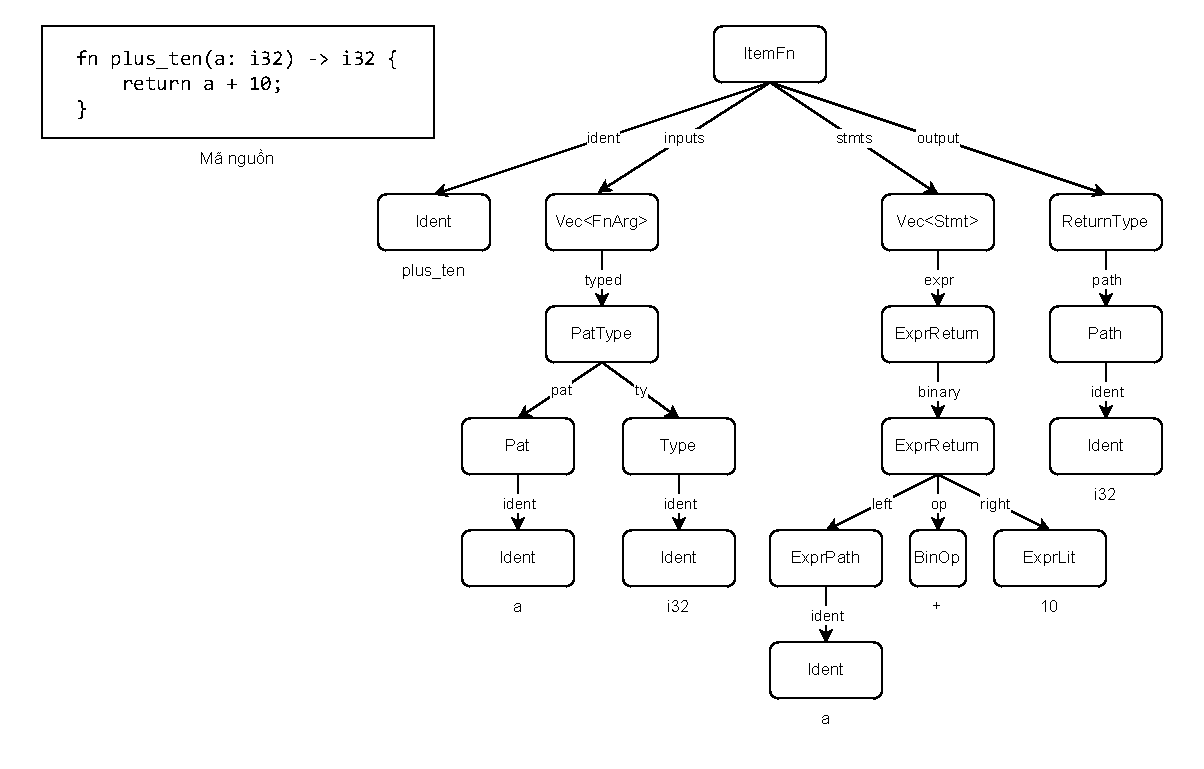
\includegraphics[width=1\columnwidth]{figures/c2/c2_ast.drawio.pdf}
  \centering
  \caption{Ví dụ về cây cú pháp trừu tượng cho mã nguồn Rust.}
  \label{img:c2_ast}
\end{figure}

\subsection{Đồ thị dòng điều khiển}

Đồ thị dòng điều khiển (Control Flow Graph) \cite{yan2019classifying} là đồ thị có hướng, biểu diễn kịch bản thực thi của chương trình/đơn vị chương trình.
Đồ thị này được xây dựng từ mã nguồn của chương trình, trong đó các nút là các câu lệnh/nhóm câu lệnh và các cạnh là các dòng điều khiển, thể hiện thứ tự thực hiện của câu lệnh/nhóm câu lệnh.
Tất cả các đồ thị dòng điều khiển đều có điểm xuất phát và điểm kết thúc đại diện cho trạng thái bắt đầu và trạng thái kết thúc của chương trình.
CFG bao gồm các thành phần chính là điểm xuất phát, khối xử lý, điểm quyết định, điểm nối và điểm kết thúc.

\begin{figure}[H]
  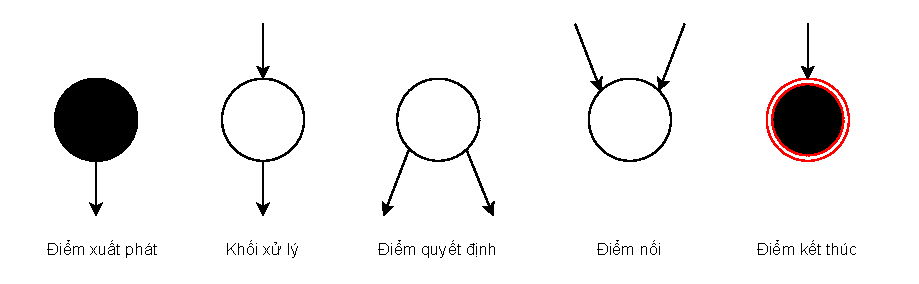
\includegraphics[width=1\columnwidth]{figures/c2/c2_cfg_point.drawio.pdf}
  \centering
  \caption{Các thành phần cơ bản trong đồ thị dòng điều khiển.}
  \label{img:c2_cfg_point}
\end{figure}

Trong hình \ref{img:c2_cfg_point}, \textbf{điểm xuất phát} và \textbf{điểm kết thúc} biểu thị điểm bắt đầu và kết thúc của chương trình, lần lượt được thể hiện bằng hình tròn đặc và hình tròn đặc viền.
\textbf{Khối xử lý} tượng trưng cho các câu lệnh gán, khai báo và khởi tạo, được thể hiện bằng hình tròn rỗng.
\textbf{Điểm quyết định} biểu thị các câu lệnh điều kiện trong các khối lệnh rẽ nhánh, được thể hiện bằng hình tròn rỗng với nhiều nhánh đi ra.
\textbf{Điểm nối} biểu thị các câu lệnh thực hiện ngay sau các lệnh rẽ nhánh, có nhiều hơn một điểm trỏ đến, được thể hiện bằng hình tròn rỗng.

\begin{figure}[H]
  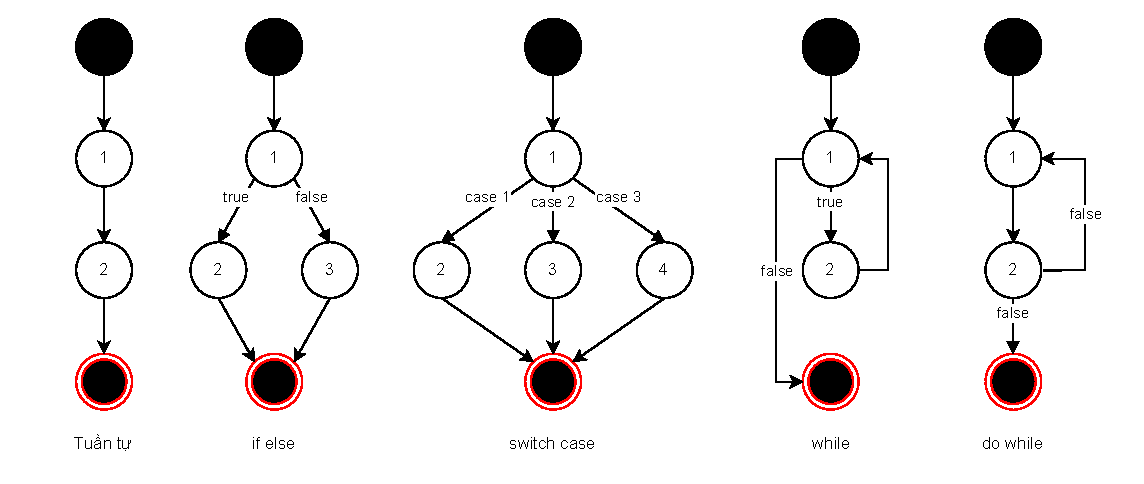
\includegraphics[width=1\columnwidth] {figures/c2/c2_cfg_line.drawio.pdf}
  \centering
  \caption{Các cấu trúc điều khiển phổ biến trong các ngôn ngữ lập trình.}
  \label{img:c2_cfg_line}
\end{figure}

Hình \ref{img:c2_cfg_line} mô tả các cấu trúc điều khiển phổ biến có trong các ngôn ngữ lập trình được biểu diễn dưới dạng đồ thị CFG, bao gồm có cấu trúc điều khiển tuần tự, $if\ else$, $switch\ case$, $while$ và $do\ while$.

\subsection{Đồ thị phụ thuộc chương trình}

% Đồ thị phụ thuộc chương trình (Program Dependence Graph) \cite{ferrante1987program, horwitz1992use} biểu diễn chương trình dưới dạng một đồ thị mà trong đó các nút là các câu lệnh và biểu thức (expression) hoặc các toán tử và toán hạng.
% Các cạnh của đồ thị biểu diễn sự phụ thuộc dữ liệu (data dependence) và điều kiện điều khiển (control condit  ion) mà việc thực thi nút đó phụ thuộc vào hay có thể hiểu đơn giản hơn là phụ thuộc điều khiển (control dependence).

% The PDG makes explicit both the data and control dependences for each operation in a program. Data dependence graphs have provided some optimizing compilers with an explicit representation of the definition-use relationships implicitly present in a source program [31, 361]. A control flow graph [1, 31] has been the usual representation for the control flow relationships of a program; the control conditions on which an operation depends can be derived from such a graph. An undesirable property of a control flow graph, however, is a fixed sequencing of operations that need not hold. The program dependence graph explicitly represents both the essential data relationships, as present in the data dependence graph, and the essential control relationships, without the unnecessary sequencing present in the control flow graph.’ These dependence relationships determine the necessary sequencing between operations, exposing potential parallelism.

% The PDG represents a program as a graph in which the nodes are statements and predicate expressions (or operators and operands) and the edges incident to a node represent both the data values on which the node’s operations depend and the control conditions on which the execution of the operations depends

Đồ thị phụ thuộc chương trình (Program Dependence Graph) \cite{ferrante1987program, horwitz1992use} là đồ thị có hướng thể hiện cả 2 khía cạnh phụ thuộc điều khiển và phụ thuộc dữ liệu của chương trình.
Một nút đại diện cho một câu lệnh / nhóm câu lệnh, một cạnh thể hiện mối quan hệ phụ thuộc điều khiển hoặc phụ thuộc dữ liệu giữa các nút.
Câu lệnh / nhóm câu lệnh mà một nút đại diện có được thực hiện hay không phụ thuộc vào các cạnh điều kiện điều khiển và điều kiện dữ liệu trỏ tới nút đó.

\begin{figure}[H]
  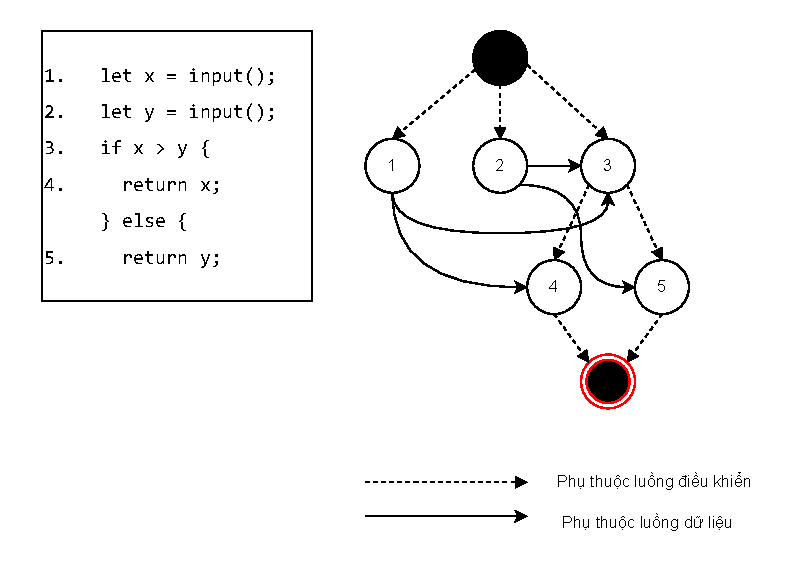
\includegraphics[width=1\columnwidth]{figures/c2/c2_pdg.drawio.pdf}
  \centering
  \caption{Ví dụ về đồ thị phụ thuộc chương trình.}
  \label{img:c2_pdg}
\end{figure}

Hình \ref{img:c2_pdg} biểu diễn ví dụ về một đồ thị phụ thuộc chương trình với cấu trúc điều kiện $if\ else$ trong ngôn ngữ Rust, các cạnh nét đứt biểu diễn phụ thuộc điều khiển và các cạnh nét liền biểu diễn phụ thuộc dữ liệu.

\subsection{Đồ thị thuộc tính mã nguồn}

Đồ thị thuộc tính mã nguồn (Code Property Graph) \cite{yamaguchi2014modeling} là một dạng đồ thị biểu diễn mã nguồn mới, được hợp thành cây cú pháp trừu tượng, đồ thị dòng điều khiển và đồ thị phụ thuộc chương trình.
Đồ thị chứa các thông tin về cấu trúc cú pháp, luồng điều khiển và phụ thuộc dữ liệu trong chương trình.
Các nút đại diện cho các thành phần như hàm, biến, lớp, gói và các cạnh đại diện cho mối quan hệ giữa chúng như lời gọi hàm, sự gán giá trị, quan hệ cha con hay tham chiếu.
CPG được sử dụng để tìm kiếm lỗ hổng trong mã nguồn, phát hiện sao chép mã nguồn, đo lường khả năng kiểm thử mã nguồn và sinh mã khai thác \cite{xiaomeng2018cpgva, han2023bjxnet, kuchler2022representing}.

\begin{figure}[H]
  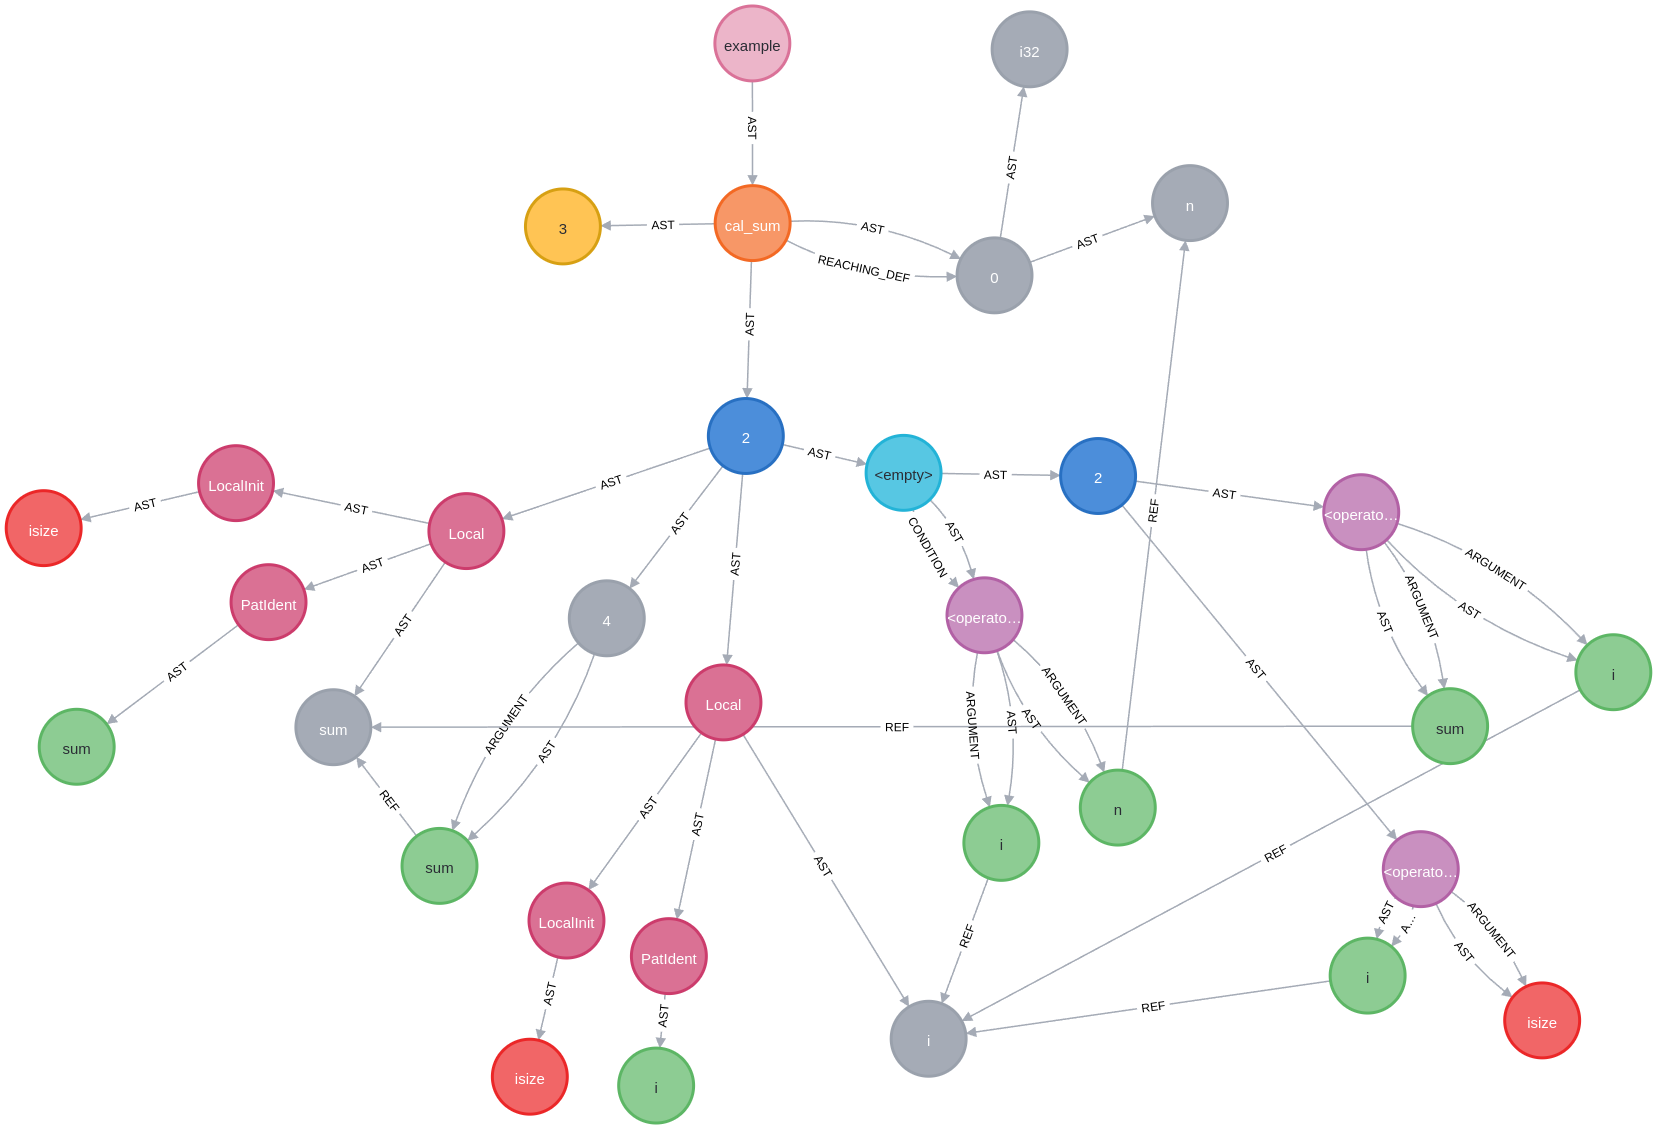
\includegraphics[width=1\columnwidth]{figures/c2/c2_cpg.png}
  \centering
  \caption{Ví dụ đồ thị thuộc tính mã nguồn.}
  \label{img:c2_cpg}
\end{figure}

\begin{listing}[H]
\begin{minted}[mathescape, breaklines, frame=lines, framesep=2mm, baselinestretch=1.2, fontsize=\footnotesize, linenos]{rust}
fn cal_sum(n: i32) {
  let mut sum = 0;
  let mut i = 1;
  while i <= n {
      sum += i;
      i += 1;
  }
  return sum;
}
\end{minted}
\caption{Mã nguồn đầy đủ cho đồ thị thuộc tính mã nguồn hình \ref{img:c2_cpg}.}
\label{code:c2_cpg}
\end{listing}
